\part{Metodologia}

\chapter[Metodologia]{Metodologia}


Este capítulo foi elaborado para melhorar o entendimento das atividades
 realizadas para a produção deste trabalho. O fluxo da figura 
\ref{fig:fases_metodologia} define estas atividades.


\begin{figure}[h]
    \centering
    \label{fig:fases_metodologia}
        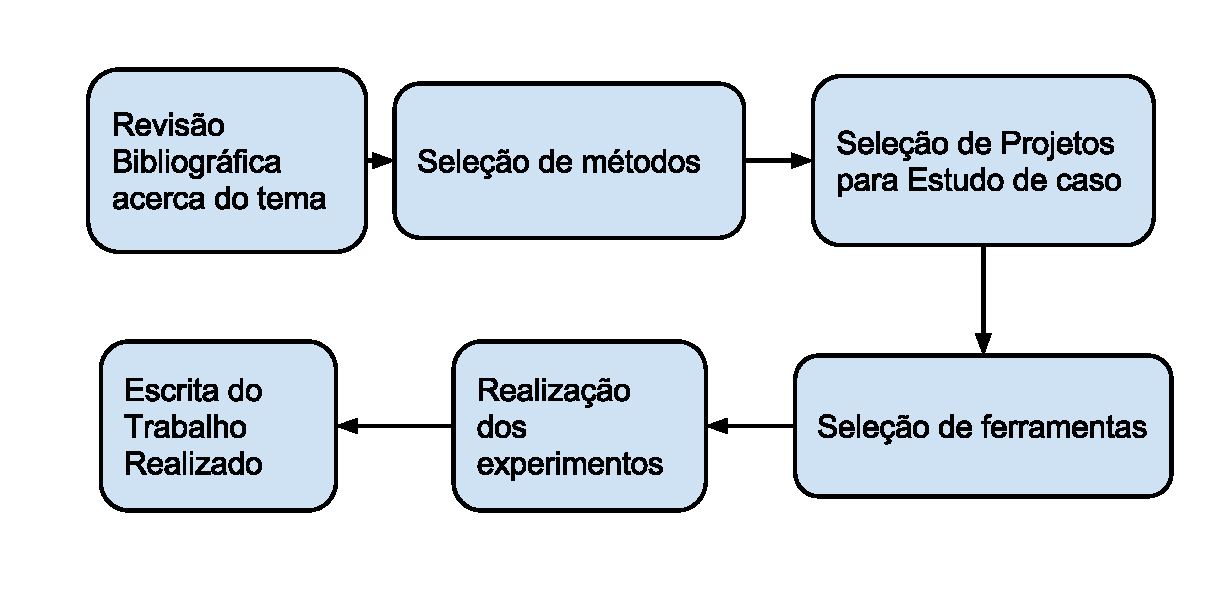
\includegraphics[keepaspectratio=true,scale=0.7]{figuras/fases_metodologia.eps}
    \caption{Fluxo de Atividades para a resolução destes trabalho}
\end{figure}


\section{Revisão Bibliográfica}

A revisão bibliográfica foi a primeira atividade realizada para a construção
 deste trabalho. Foi feito um estudo e levantamento de métodos, técnicas e
 ferramentas que podem auxiliar o desenvolvimento deste trabalho, além de
 elucidar a viabilidade da realização do mesmo. Esta revisão foi utilizada
 como referência para a  escrita da fundamentação teórica.

\section{Seleção de Métodos}

Para seleção de métodos foi realizada uma priorização dos métodos, técnicas e
 ferramentas encontradas durante a revisão bibliográfica. A priorização levou
 em conta o esforço da implementação/execução dos métodos, o tempo para a
 montagem de experimentos e o recurso computacional necessário para a criação
 destes experimentos.


Os métodos selecionados foram:

\begin{enumerate}
	\item Include Guards, descrito na seção
 \ref{include_guards_section};
	\item Forward Declaration, descrito na seção
 \ref{forward_declaration_section};
	\item Makefile, descrito na seção
 \ref{Makefile_section};
	\item Otimização de baixo nível;
	\item Pimpl Idiom;
	\item Compilador + Headers pré-compilados;
	\item Ferramentas que utilizam cache de arquivos 
pré-processados (CCache, Wrap, Gold);
\end{enumerate}

\section{Seleção de Projetos}

Para a realização dos experimentos  envolvendo os métodos selecionados na
 atividade anterior foi feita uma busca de possíveis softwares livres que
 poderiam ser modificados.  As modificações seriam realizadas com o intuito
 de conseguir diferenciar o tempo de compilação de um projeto com a aplicação
 de algum dos métodos selecionados e sem  esta aplicação. Além das
 modificações, foram criados scripts para auxiliar a execução de experimentos
 que automatizassem a compilação e medissem o tempo gasto.

\subsection{Critérios de Seleção}


Para a seleção dos projetos aqui presentes foram feitos filtros de pesquisas
 na plataforma Github\footnote{Github: http://github.com.}. Para o presente
 trabalho foram escolhidos primeiramente os 3 primeiros métodos para estudo,
 e que deveriam ser aplicados em projetos com mais de 50\% do código fonte em
 C++. Para garantir isso, foi utilizado a ferramenta sloccount para realizar
 a contagem de linhas do projeto e a percentagem de código em C++.
 A Tabela \ref{tab:projects} mostra os projetos selecionados e quais métodos
 poderiam ser aplicados.

\begin{table}[h]
\centering
\begin{tabular}{|l|p{2cm}|p{2cm}|p{2cm}|p{2cm}|p{2cm}|}
	\hline
	Projetos & Quantidade de linhas do projeto & Porcentagem em C++ &
	Guarda de Inclusão & Forward declaration & Makefile \\
	\hline
	cppcheck & 136,906 & (96.02\%) & Não & Não & Sim \\
	\hline
	hayai & 1,668 & (83.27\% & Não & Não & Sim \\
	\hline
	jsoncpp & 9,833 & 80.21\% & Não & Não & Sim \\
	\hline
	libsass & 21,962 & 93.79\% & Não & Não & Sim \\
	\hline
	libOauthCpp & 2,128 & 87.27\% & Não & Não & Sim \\
	\hline
	Jack, the Janitor & 2,062 & 99.22\% & Não & Sim & Sim \\
	\hline
\end{tabular}
\caption{Projetos e Métodos que podem ser aplicados}
\label{tab:projects}
\end{table}

\subsection{Projetos Selecionados}

Foram selecionados 5 projetos: cppcheck, hayai, jsoncpp, libsass,
 libOAuthcpp e Jack ,the Janitor. Este projetos serão brevemente 
descritos a seguir.

\textbf{CppCheck} é uma ferramenta de código de C/C++, que detecta erros no código
 que compiladores e outras ferramentas não detectariam . Este projeto realiza
 as seguintes verificações \footnote{CppCheck: http://cppcheck.sourceforge.net/
  acessado em 17/06/2015.}:

\begin{itemize}
	\item Índice fora dos limites do vetor;    
    \item Vazamentos de memória;
    \item Possíveis deferências ponteiro nulo ( o que causa falhas de segmentação);
	\item Existência de variáveis não inicializadas;
	\item Uso inválido da STL;
	\item Funções obsoletas ou com falhas de segurança; 
	\item código não utilizado ou redundante;
	\item Entre outros;
\end{itemize}


\textbf{Hayai}\footnote{Hayai: https://github.com/nickbruun/hayai acessado em
 17/06/2015.} é um framework para realização de benchmark em C++,utilizados
 para testes de unitários usando googletest.

\textbf{JsonCpp} \footnote{Jsoncpp: https://github.com/nickbruun/hayai acessado
 em 17/06/2015. } é uma biblioteca que permite a manipulação de arquvios .json,
 incluindo serialização e deserialização de strings. Esta pode preservar
 comentários existentes na serialização/deserialização, tornando-se um formato
 conveniente para armazenar de entradas de usuário.

\textbf{LibSass} \footnote{LibSass: https://github.com/sass/libsass acessado
 em 17/06/2015.} é uma ferramenta de pré-processamento de Sass Css. Esta
 ferramenta foi originalmente criada em Ruby, no entanto a versão aqui utilizada
 é mais simples, leve, eficiente e portátil.

\textbf{LibOAuthCpp} \footnote{LibOAuthCpp: https://github.com/sirikata/liboauthcpp
 acessado em 17/06/2015} é uma biblioteca de C++ voltada para realizar solicitações
 de autenticação utilizando o protocolo OAuth. Ela não implementa solicitações de
 requisições em HTTP mas, no entanto, é utilizada como uma interface de suporte ao
 OAuth.

\textbf{Jack, the Janitor} \footnote{Jack, the Janitor: https://github.com/athos-ribeiro/jtj
 acessado em 17/06/2015;} é um jogo onde o jogador controla  a personagem Jack,
 o zelador de uma escola, que deve organizar o armazém da escola. Jack pode empurrar
 caixas para esquerda, para a direita ou saltar.O objetivo do jogo e preencher uma
 linha inteira de caixas: caso Jack seja atingido por uma caixa o jogo é finalizado
 com \textit{gameover}.

\section{Ferramentas}

As linguagens utilizadas foram C++ versão 11 e Python versão +2.7.

Para realiazar a contagem do tempo foi utilizado o programa Time.
 Programa escrito por David MacKenzie e tem como objetivo indicar o tempo gasto
 por um processo em diferentes aspectos.
 O comando time tem como saída 3 tipos de valores:

\begin{itemize}
	\item User: É o tempo gasto por um processo em modo usuário;
	\item System:  É o tempo gasto por um processo em modo kernel;
	\item Real:  É o tempo total gasto na execução de um processo;
\end{itemize}

Para a coleta dos tempos foi utilizado apenas o valor Real, uma vez que este
 expressa o tempo total decorrido para a realização de um processo.

O compilador escolhido para o trabalho foi o g++. O g++ é uma melhoria do
 compilador gcc, criado pela GNU, que possui com conjunto de ferramentas
 para realiza pré-processamento , compilação, montagem e linkedição.
 No front-end,  este compilador inclui as linguagens C, C++, Objective-C,
 Fortran, Java, Ada, and Go, bem como as suas bibliotecas  (libstdc++,
 libgcj, entre outras)\footnote{GCC\_GNU: https://gcc.gnu.org/ acessado
 em 17/06/2015}.


Os experimentos realizados foram feitos utilizando um computador pessoal
 (notebook), com  as especificações  listadas na Tabela 
\ref{tab:especificacoes_hardware}.


\begin{table}[h]
\centering
\begin{tabular}{|l|l|}
	\hline
	Processador         & Intel i7 2.0Ghz \\
	\hline
	Memória RAM         & 6GB             \\
	\hline
	Placa de Rede       & Sim             \\
	\hline
	Sistema Operacional & Ubuntu 15.04 \\
	\hline
\end{tabular}
\caption{Especificações do computador utilizado.}
\label{tab:especificacoes_hardware}
\end{table}


Apesar de ser um computador pessoal, uma maquina virtual utilizando Virtualbox
 foi criada para realizar um independência entre a máquina pessoal e os
 arquivos e programas pessoais, além de uma melhora  na visualização da
 diferença de tempo de compilação entre projetos
 \footnote{No caso de projetos menores e de compilação mais rápida, pois o 
\textit{overhead} proveninte da execução da máquina virtual torna os tempos
 absolutos de compilação maiores do que na máquina host}, independente do
 tamanho do projeto. As especificação da máquina virtual  estão listadas na
 Tabela \ref{tab:especificacoes_vm}.

\begin{table}[h]
	\centering
	\begin{tabular}{|l|l|}
		\hline
		Processador & 2 PCUs \\
		\hline
		Memória RAM & 3 GB \\
		\hline
		Memória ROM & 8 GB \\
		\hline
		Placa de Rede & Sim \\
		\hline
		Sistema Operacional & Ubuntu 14.04 \\
		\hline
		VirtualBox & 4.3.26\_Ubuntu \\
		\hline
	\end{tabular}
	\caption{Especificações máquina virtual utilizada}
	\label{tab:especificacoes_vm}
\end{table}


\section{Montagem dos experimentos/scripts}

Para a primeira etapa deste trabalho foram escolhidos 3 experimentos a
 serem aplicados.

\textbf{Experimento 1}:\label{experimento_1}

Para a realização de experimentos com Inclusão de Guarda foram elaborados
 em scripts Python que criam projetos simples com a inclusão de cabeçalhos
 três vez e com diferentes tipos de inclusão, como mostrado na  Seção
 \ref{include_guards_section}.
 No apêndice geração de prjetos é apresentado estes scripts.

O script cria uma pasta chamada include e, dentro dela, arquivos com o padrão
 <NUMERO>.hpp, que são os cabeçalhos a serem incluídos no arquivo main.cpp.
 Foram criados 10 mil arquivos. Os Códigos \ref{codigo_27} e  \ref{codigo_28}
 referenciam estes modelos.



\begin{lstlisting}[language=C++,frame=single,captionpos=b,caption={Modelo de
									 Arquivo .hpp gerado pelos scripts de 
									  guardas de inclusão},
                                                   label=codigo_27]

  // <NUMERO>.hpp

  const int int<NUMERO> = <NUMERO>;

\end{lstlisting}



\begin{lstlisting}[language=C++,frame=single,captionpos=b,caption={Modelo de
                               Arquivo main.cpp criado pelos scripts de
                                                     guardas de inclusão},
                                                          label=codigo_28]

    // main.cpp

    /* headers a serem incluidos   */

    ...


    int main(){return 0;}

\end{lstlisting}




Os scripts abordam os métodos:

\begin{itemize}
	\item Guarda de Inclusão Externa;
	\item Guarda de Inclusão Interna;
	\item Pragma Once;
	\item Guarda de Inclusão Interna primeiro que Pragma Once;
	\item Pragma Once primeiro que  Guarda de Inclusão Interna;
	\item Guarda de Inclusão Externa + Pragma Once;
	\item Redundância de Guarda de Inclusão;
\end{itemize}


A Tabela \ref{tab:modelo_guards} representa o modelo utilizado na coleta dos
 dados.


\begin{table}[h]
\centering
\begin{tabular}{|l|p{1.5cm}|p{1.5cm}|p{1.5cm}|p{1.5cm}|p{2cm}|p{2cm}|p{2cm}|p{2cm}|}
\hline
Tipo & \multicolumn{7}{l|}{Utilização de Guarda de Inclusão} \\ \hline
Medida & \multicolumn{7}{l|}{Tempos em segundos } \\ \hline
Amostras & Guarda de Inclusão Extena & Guarda de Inclusão Interna & Pragma Once & Guarda de Inclusão Interna Primeiro que Pragma Once & Pragma Once primeiro que Guarda de Inclusão Interna & Guarda de Inclusão Externa e Pragma Once & Redundancia de Guarda de Inclusão \\ \hline
 1  &  &  &   &   &   &  & \\ \hline
 2  &  &  &   &   &   &  & \\ \hline
 3  &  &  &   &   &   &  & \\ \hline
 4  &  &  &   &   &   &  & \\ \hline
 5  &  &  &   &   &   &  & \\ \hline
 6  &  &  &   &   &   &  & \\ \hline
 7  &  &  &   &   &   &  & \\ \hline 
 8  &  &  &   &   &   &  & \\ \hline
 9  &  &  &   &   &   &  & \\ \hline
 10 &  &  &   &   &   &  & \\ \hline
 Média: &  &  & & &   &  & \\ \hline
\end{tabular}
\caption{Template de amostra de Guardas de Inclusão}
\label{tab:modelo_guards}
\end{table}


\textbf{Experimento 2}:

O segundo experimento utilizou o projeto Jack, the Janitor, no qual foi
 realizada uma refatoração dos cabeçalhos: foram incluídas forward
 declarations, os headers transferidos para o arquivo de
 implementação. Após estas modificações foi feito testes com o comando
 time e o makefile do projeto. Os valores obtidos foram armazenados no
 modelo mostrado na Tabela \ref{tab:modelo_forward_declaration}

\begin{table}[h]
\centering
\begin{tabular}{|l|p{3cm}|p{3cm}|p{3cm}|}
\hline
Tipo       & \multicolumn{3}{l|}{Forward Declaration}                                                                                                                            \\ \hline
Tempo      & \multicolumn{3}{l|}{Em segundos}                                                                                                                                    \\ \hline
Repetições & Tempo de Compilação SEM forward Declaration & Tempo de Compilação COM Forward Declaration & Fator de Redução) \\ \hline
1 &  &  &  \\ \hline
2 &  &  &  \\ \hline
3 &  &  &  \\ \hline
4 &  &  &  \\ \hline
5 &  &  &  \\ \hline
6 &  &  &  \\ \hline
7 &  &  &  \\ \hline
8 &  &  &  \\ \hline
9 &  &  &  \\ \hline
10 &  &  &  \\ \hline
Média &  &  &  \\ \hline
\end{tabular}
\caption{Template para amostras com Forward Declaration}
\label{tab:modelo_forward_declaration}
\end{table}



Experimento 3: \label{experimento_03}

Realizar um estudo da redução do tempo de compilação utilizando o comando
 mostrado no Código \ref{codigo_29} que permite a compilação em
 mútliplas threads.


\begin{lstlisting}[language=C++,frame=single,captionpos=b,caption={Execução programa 
								time mais programa make executando com threads},
                                                  			 label=codigo_29]

        $ time make -j N
\end{lstlisting}

Os valores foram colocados no modelo mostrado na Tabela \ref{tab:makefile},
 com o tempo em segundos.

\begin{table}[h]
\centering
\begin{tabular}{|p{1cm}|p{1.4cm}|p{1.4cm}|p{1.4cm}|p{1.4cm}|p{1.4cm}|p{1.4cm}|p{1.4cm}|p{1.4cm}|p{1.4cm}|}
\hline
Projeto               & \multicolumn{9}{l|}{Hayai}        \\ \hline
Tempo                 & \multicolumn{9}{l|}{Em segundos}      \\ \hline
Quantidade de Threads & 1 & 2 & 4 & 6 & 8 & 10 & 12 & 14 & 16 \\ \hline
Repetições            & - & - & - & - & - & -  & -  & -  & -  \\ \hline
1 &  &  &  &  &  &  &  &  &  \\ \hline
2 &  &  &  &  &  &  &  &  &  \\ \hline
3 &  &  &  &  &  &  &  &  &  \\ \hline
4 &  &  &  &  &  &  &  &  &  \\ \hline
5 &  &  &  &  &  &  &  &  &  \\ \hline
6 &  &  &  &  &  &  &  &  &  \\ \hline
7 &  &  &  &  &  &  &  &  &  \\ \hline
8 &  &  &  &  &  &  &  &  &  \\ \hline
9 &  &  &  &  &  &  &  &  &  \\ \hline
10 &  &  &  &  &  &  &  &  &  \\ \hline
Média &  &  &  &  &  &  &  &  &  \\ \hline
\end{tabular}
\caption{Template para amostras de Makefile}
\label{tab:makefile}
\end{table}


